%=======================02-713 LaTeX template, following the 15-210 template==================
%
% You don't need to use LaTeX or this template, but you must turn your homework in as
% a typeset PDF somehow.
%
% How to use:
%    1. Update your information in section "A" below
%    2. Write your answers in section "B" below. Precede answers for all 
%       parts of a question with the command "\question{n}{desc}" where n is
%       the question number and "desc" is a short, one-line description of 
%       the problem. There is no need to restate the problem.
%    3. If a question has multiple parts, precede the answer to part x with the
%       command "\part{x}".
%    4. If a problem asks you to design an algorithm, use the commands
%       \algorithm, \correctness, \runtime to precede your discussion of the 
%       description of the algorithm, its correctness, and its running time, respectively.
%    5. You can include graphics by using the command \includegraphics{FILENAME}
%
\documentclass[11pt]{article}
\usepackage{amsmath,amssymb,amsthm}
\usepackage{tikz}
\usetikzlibrary{arrows,positioning, calc}
\tikzstyle{vertex}=[draw,fill=black!15,circle,minimum size=20pt,inner sep=0pt]
\usepackage{graphicx}
\usepackage[margin=1in]{geometry}
\usepackage{fancyhdr}
\usepackage{mathtools}
\usepackage{placeins}
\usepackage{listings}
\usepackage{color}

\definecolor{dkgreen}{rgb}{0,0.6,0}
\definecolor{gray}{rgb}{0.5,0.5,0.5}
\definecolor{mauve}{rgb}{0.58,0,0.82}

\lstset{frame=none,
  language=Java,
  aboveskip=3mm,
  belowskip=3mm,
  showstringspaces=false,
  columns=flexible,
  basicstyle={\small\ttfamily},
  numbers=none,
  numberstyle=\tiny\color{gray},
  keywordstyle=\color{blue},
  commentstyle=\color{dkgreen},
  stringstyle=\color{mauve},
  breaklines=true,
  breakatwhitespace=true,
  tabsize=3
}

\setlength{\parindent}{0pt}
\setlength{\parskip}{5pt plus 1pt}
\setlength{\headheight}{13.6pt}
\newcommand\question[2]{\vspace{.25in}\hrule\textbf{#1 #2}\vspace{.5em}\hrule\vspace{.10in}}
\renewcommand\part[1]{\vspace{.10in}\textbf{(#1)}}
\newcommand\algorithm{\vspace{.10in}\textbf{Algorithm: }}
\newcommand\correctness{\vspace{.10in}\textbf{Correctness: }}
\newcommand\runtime{\vspace{.10in}\textbf{Running time: }}
\pagestyle{fancyplain}
\lhead{\textbf{\NAME}}
\chead{\textbf{HW\HWNUM}}
\rhead{\today}
\begin{document}\raggedright
%Section A==============Change the values below to match your information==================
\newcommand\NAME{Sean Connor}  % your name
\newcommand\HWNUM{6}              % the homework number
%Section B==============Put your answers to the questions below here=======================

\question{Q1}{}
A node at level n has exactly n ancestors, assuming root node is level zero. This is because each node (except for the root node) has one parent node. So a node at level one has a single parent, the root node. A node at level two has a parent at level one, who has a parent at level zero, and so on.

\begin{center}
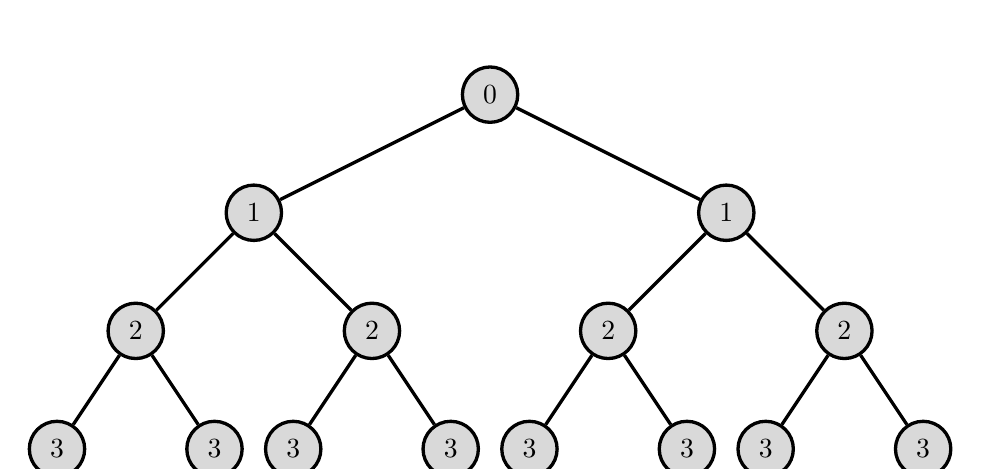
\begin{tikzpicture}[very thick,level/.style={sibling distance=60mm/#1}]
\node [vertex] (r){$0$}
	child {node [vertex] (a) {$1$}
		child {node [vertex] {$2$}
      			child {node [vertex] {$3$}}
      			child {node [vertex] {$3$}}
			}		
		child {node [vertex] {$2$}
      			child {node [vertex] {$3$}}
      			child {node [vertex] {$3$}}
			}
		}
	child {node [vertex] (a) {$1$}
		child {node [vertex] {$2$}
      			child {node [vertex] {$3$}}
      			child {node [vertex] {$3$}}
			}
		child {node [vertex] {$2$}
      			child {node [vertex] {$3$}}
      			child {node [vertex] {$3$}}
			}
		};
\end{tikzpicture}
\end{center}

\question{Q2}{}
Assume that the number of nodes is given by $2n-1$ where n is the number of leaves of a binary tree. If there is a binary tree of level zero, there will be a single leaf. By the previous equation, $2(1)-1 = 1$, and so the equation is satisfied. 

If a binary tree T has two children, subtrees A and B, then the total number of leaves will be $leaves_A + leaves_B = leaves_T$, or $a + b = t$. By the previous equation, A and B each have $2a-1$ and $2b-1$ nodes, respectively. Thus, the total number of nodes in T is $1+(2a-1)+(2b-1)$.
\begin{align*}
1+(2a-1)+(2b-1) = \\
1+2a+2b-2 = \\
2a+2b-1 = \\
2(a+b)-1 = \\
2t-1 = \\
\fbox{$2n-1$}
\end{align*}

\question{Q3}{}
The total number of pointer fields will be equal to the number of nodes times the number of pointer fields per node. For an m-ary tree, this will be equal to $n\times m$. All nodes except for the primary root node have a pointer from their parent node. Thus the number of ``allocated" pointers is $n-1$. The number of remaining null pointers is thus equal to $(n\times m)-(n-1)$. Simplifying, we see:
\begin{align*}
 (n\times m)-(n-1) = \\
(n\times m) - n + 1 = \\
nm - n + 1 = \\
\fbox{$n(m-1)+1$}
\end{align*}

\question{Q4}{}
\begin{lstlisting}
/** Java/pseudocode for right in-thread binary tree with  
 ** sequential array representation
 */

// class to represent a node in the tree
class Node{
	DataType data;
	int left;	// int value representing index of left node
	int right;	// int value representing index of right node
	boolean rThread;
}

// binary tree class (sequential array implementation)
public class TreeClass{
	private Node[] treeArray;

	// constructor
	public void TreeClass(int size, DataType item){
		treeArray = new Node[size];
		treeArray[0] = makeTree(item);
	}

	// returns true if tree is empty, false otherwise
	public boolean isEmpty(){
		if (treeArray[0] == null){
			return true;
		} else{
			return false;
		}
	}

	//  creates a new node with data, null left and right pointers, and rThread = false
	public void makeTree(DataType item){
		Node temp = new Node;
		temp.data = item;
		temp.left = null;
		temp.right = null;
		temp.rThread = false;
		return temp;
		
	}

	// creates a left child node with data
	public void setLeft(int parentIndex, DataType item){
		Node p = treeArray[parentIndex];
		int childIndex = 2 * parentIndex; // set correct index for child
		if (p == null) {
			throw exception;
		} 
		else if (p.left != null){
			throw exception;
		}
		else{
			Node temp = makeTree(item);
			p.left = childIndex;
			temp.right = parentIndex;
			temp.rThread = true;
			treeArray[childIndex] = temp; // place new node at appropriate location in array
		}
	}

	// creates a right child node with data
	public void setRight(int parentIndex, DataType item){
		Node p = treeArray[parentIndex];
		int childIndex = 2 * parentIndex + 1; // set correct index for child 
		if (p == null) {
			throw exception;
		} 
		else if (!p.rThread){
			throw exception;
		}
		else{
			Node temp = makeTree(item);
			temp.right = p.right;
			temp.rThread = true;
			p.right =  childIndex;
			p.rThread = false;
			treeArray[childIndex] = temp; // place new node at appropriate location in array
		}
	}

}
\end{lstlisting}

\question{Q5}{}
The traverse can be easily accomplished using a recursive method.
\begin{lstlisting}
/* Java/pseudocode for in-order traversal of sequential array binary tree */

public void traverse(int index){
 	if (treeArray[index] != null){ 	// if index/node is null, do nothing
		int lc = 2*index;		// set left child index
		int rc = lc+1;			// set right child index
		traverse(lc);			// recursively call traverse() on left child
		System.out.println(treeArray[index].data);
		traverse(rc);			// recursively call traverse() on right child
	}
}
\end{lstlisting}

\question{Q6}{}
This is easily accomplished by using a recursive method to create a Fibonacci subtree at the right and left children/pointers for every order greater than or equal to two. Order one and order zero are base cases in this method.
\begin{lstlisting}
/* Java/pseudocode for a Fibonacci binary tree */

// Node object used for creating Fibonacci tree
class Node{
	int data;
	Node left;
	Node right;
}

// method for creating a Fibonacci binary tree of specified order
public fibTree(int order){
	if (order == 0){
		Node temp = new Node();
		temp.data = order;
		temp.left = null;
		temp.right = null;		
	}
	else if (order == 1){
		Node temp = new Node();
		temp.data = order;
		temp.left = null;
		temp.right = null;
	} 
	else {
		Node temp = new Node();
		temp.data = order;
		temp.left = fibTree(order-1);
		temp.right = fibTree(order-2);
	}
}
\end{lstlisting}

As an example, if fibTree(3) was called, the result would be:

\begin{center}
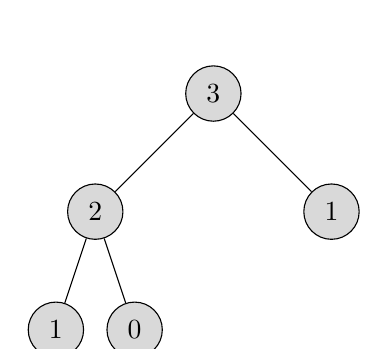
\begin{tikzpicture}[every node/.style={circle,draw},level 1/.style={sibling distance=30mm},level 2/.style={sibling distance=10mm}]
\node [vertex] (r){$3$}
	child {node [vertex] (a) {$2$}
		child {node [vertex] {$1$}}
      		child {node [vertex] {$0$}}
		}
	child {node [vertex] (a) {$1$}};
\end{tikzpicture}
\end{center}

\question{Q7}{}
\part{a} 
A Fibonacci tree does not need to be binary. Any m-ary tree will work. There will be m base cases. For example, here is a ternary Fibonacci tree.

\begin{center}
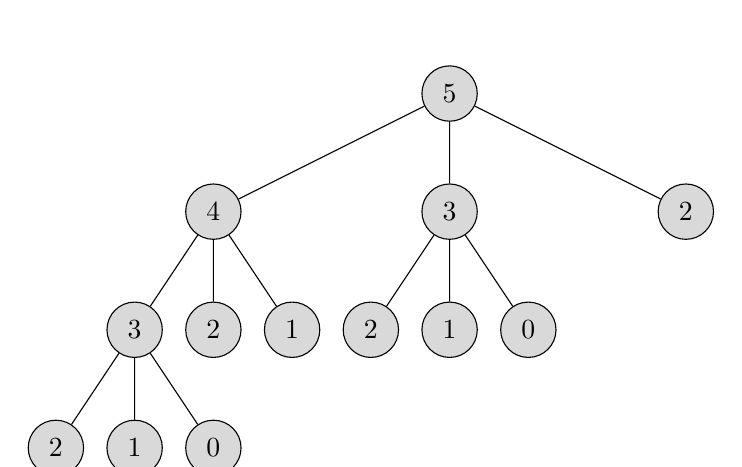
\begin{tikzpicture}[every node/.style={circle,draw},level 1/.style={sibling distance=30mm},level 2/.style={sibling distance=10mm}]
\node [vertex] (r){$5$}
	child {node [vertex] (a) {$4$}
		child {node [vertex] {$3$}
			child {node [vertex] {$2$}}
			child {node [vertex] {$1$}}
			child {node [vertex] {$0$}}
			}
      		child {node [vertex] {$2$}}
		child {node [vertex] {$1$}}
		}
	child {node [vertex] (a) {$3$}
		child {node [vertex] {$2$}}
      		child {node [vertex] {$1$}}
		child {node [vertex] {$0$}}
	}
	child {node [vertex] (a) {$2$}};
\end{tikzpicture}
\end{center}

\part{b}
The number of leaves is given by the following:
\begin{align*}
\# leaves_n = \# leaves_{n-1} + \# leaves_{n-2}
\end{align*}
Alternatively,
\begin{align*}
\# leaves_n = fibonacci(n+1)
\end{align*}

\part{c}
The depth of the tree (assuming binary, depth starts at 0) is simply $n-1$.

\end{document}









